\documentclass[nofootinbib,notitlepage,11pt]{revtex4-2}

%%% linking references
\usepackage{hyperref}
\hypersetup{
  breaklinks=true,
  colorlinks=true,
  linkcolor=blue,
  filecolor=magenta,
  urlcolor=cyan,
}

%%% header / footer
\usepackage{fancyhdr} % easier header and footer management
\pagestyle{fancy} % page formatting style
\fancyhf{} % clear all header and footer text
\renewcommand{\headrulewidth}{0pt} % remove horizontal line in header
\usepackage{lastpage} % for referencing last page
\cfoot{\thepage~of \pageref{LastPage}} % "x of y" page labeling

%%% symbols, notations, etc.
\usepackage{physics,braket,bm,amssymb} % physics and math
\renewcommand{\t}{\text} % text in math mode
\newcommand{\f}[2]{\dfrac{#1}{#2}} % shorthand for fractions
\newcommand{\p}[1]{\left(#1\right)} % parenthesis
\renewcommand{\sp}[1]{\left[#1\right]} % square parenthesis
\renewcommand{\set}[1]{\left\{#1\right\}} % curly parenthesis
\newcommand{\bk}{\Braket} % shorthand for braket notation

\renewcommand{\c}{\cdot} % inner product

\newcommand{\m}{\bm} % bold symbol
\renewcommand{\v}{\vec} % arrow vector

\usepackage{dsfont} % for identity operator
\newcommand{\1}{\mathds{1}}

\newcommand{\up}{\uparrow}
\newcommand{\dn}{\downarrow}

\renewcommand{\d}{\text{d}}
\newcommand{\x}{\text{x}}
\newcommand{\y}{\text{y}}
\newcommand{\z}{\text{z}}

\newcommand{\A}{\mathcal{A}}
\newcommand{\B}{\mathcal{B}}
\newcommand{\C}{\mathcal{C}}
\newcommand{\D}{\mathcal{D}}
\newcommand{\E}{\mathcal{E}}
\newcommand{\G}{\mathcal{G}}
\newcommand{\I}{\mathcal{I}}
\renewcommand{\L}{\mathcal{L}}
\newcommand{\M}{\mathcal{M}}
\newcommand{\N}{\mathcal{N}}
\renewcommand{\O}{\mathcal{O}}
\renewcommand{\P}{\mathcal{P}}
\renewcommand{\S}{\mathcal{S}}
\newcommand{\T}{\mathcal{T}}

\newcommand{\PP}{\mathbb{P}}
\renewcommand{\SS}{\mathbb{S}}
\newcommand{\TT}{\mathbb{T}}
\newcommand{\ZZ}{\mathbb{Z}}

\newcommand{\PS}{\text{PS}}
\newcommand{\EQPS}{=_{\text{PS}}}
\newcommand{\col}{\underline}

\let\var\relax
\DeclareMathOperator{\var}{var}
\DeclareMathOperator{\cov}{cov}
\DeclareMathOperator{\diag}{diag}
\newcommand{\ul}{\underline}

\usepackage{accents} % for the undertilde
\newcommand{\ut}{\undertilde}

\newcommand{\lra}{\leftrightarrow}
\newcommand{\floor}[1]{\lfloor{#1}\rfloor}

\usepackage[inline]{enumitem} % in-line lists and \setlist{} (below)
\setlist[enumerate,1]{label={(\roman*)}} % default in-line numbering
\setlist{nolistsep} % more compact spacing between environments

%%% figures
\usepackage{graphicx} % for figures
\graphicspath{{./figures/}} % set path for all figures
\usepackage[export]{adjustbox} % for vertical alignment in math
\newcommand{\diagram}[1]
{\,\includegraphics[valign=c]{diagrams/#1.pdf}\,}

% alphanumeric footnotes
\renewcommand*{\thefootnote}{\alph{footnote}}

% for energy diagrams, etc.
\usepackage{tikz}
\usetikzlibrary{arrows,math}
\tikzstyle{every picture}+=[remember picture]

%%% text markup
\usepackage{color} % text color
\newcommand{\red}[1]{{\color{red} #1}}

%%%%%%%%%%%%%%%%%%%%%%%%%%%%%%%%%%%%%%%%%%%%%%%%%%%%%%%%%%%%%%%%%%%%%%
\begin{document}

\title{SU($n$) spin models near the Heisenberg critical point}%
\author{Michael A. Perlin}%
\date{\today}

\maketitle

\tableofcontents

\section{Introduction}

\red{TODO: write an introduction}

%%%%%%%%%%%%%%%%%%%%%%%%%%%%%%%%%%%%%%%%%%%%%%%%%%%%%%%%%%%%%%%%%%%%%%
\section{The SU($n$) Heisenberg model}

We consider an array of $N$ multilevel spins with SU($n$)-symmetric
interactions that can be written in the form
\begin{align}
  H_0 = \sum_{\set{p,q}\in\C_N\p{2}} h_{pq} \Pi_{pq},
  &&
  \Pi_{pq} \equiv \sum_{\mu,\nu\in\ZZ_n} s_{\mu\nu}^{(p)} s_{\nu\mu}^{(q)},
  \label{eq:H_0}
\end{align}
where $p,q$ index individual spins; $\C_N\p{2}$ is the set of all
subsets (``choices'') of two spins out of $N$; $h_{pq}$ are scalar
coupling constants; $\mu,\nu$ index states in an orthonormal basis for
the $n$-dimensional Hilbert space of a single spin; $\ZZ_n$ is the set
of integers modulo $n$; the operator
$s_{\mu\nu}^{(p)}\equiv\op{\mu}{\nu}_p$ flips the state of spin $p$ to
$\ket\nu$ from $\ket\mu$; and the operator $\Pi_{pq}$ permutes the
states of spins $p$ and $q$.  The permutation operator $\Pi_{pq}$ is
essentially a multilevel generalization of the SU(2)-symmetric spin
interaction $\v s_p\c\v s_q$, with $\v s\equiv\p{\v s_\x,s_\y,s_\z}$,
$s_\alpha\equiv\sigma_\alpha/2$, and $\sigma_\alpha$ a single-spin
Pauli operator.

If the coefficients $h_{pq}$ of the interaction Hamiltonian $H_0$ are
all negative, then the ground-state manifold $\M_0$ of the interaction
Hamiltonian $H_0$ consists of permutationally symmetric (PS) states
that are simultaneous $+1$ eigenstates of all permutation operators
$\Pi_{pq}$.  We will assume that all $h_{pq}<0$ throughout these
notes, but note that this restriction can be relaxed to the assumption
that the initial state of all spins is permutationally symmetric
(e.g.~a spin-polarized state).  We will also assume that the PS
manifold $\M_0$ is gapped away from all orthogonal states by an
interaction energy $\Delta_{\t{gap}}>0$.  Power-law couplings of the
form $h_{pq}\sim-1/\abs{p-q}^\alpha$ on a $D$-dimensional lattice, for
example, always yield a non-vanishing spectral gap $\Delta_{\t{gap}}$
for long-range interactions with $\alpha\le D$ (see Appendix
\ref{sec:spectral_gap}).

The PS manifold $\M_0$ is spanned by a basis of states
$\ket{m}=\ket{m_1,m_2,\cdots,m_n}$ with a definite occupation number
$m_\mu$ of the single-spin state $\mu$, and $\sum_\mu m_\mu=N$.  We
denote the set of all such assignments of $N$ (identical) spins to $n$
(distinct) states by $\A_n\p{N}$, such that our standard basis for
$\M_0$ is $\set{\ket{m}:m\in\A_n\p{N}}$.  The dimension of $\M_0$ is
then the number of such assignments, which is straightforward to
determine with a standard ``stars and bars'' calculation:
$\abs{\A_n\p{N}} = {N+n-1 \choose n-1} \sim N^{n-1}$.  In the case of
$n=2$, for example, the PS manifold $\M_0$ is precisely the Dicke
manifold\cite{dicke1954coherence} of $N$ qubits, spanned by
${N+2-1\choose2-1}=N+1$ Dicke states $\ket{m_0,m_1}$ for which
$m_0+m_1=N$ and the integer $m_0$ ($m_1$) indicates the total
occupation number of qubit state $\ket{0}$ ($\ket{1}$).  The energy of
any PS state $\ket\psi\in\M_0$ with respect to the interaction
Hamiltonian $H_0$ in \eqref{eq:H_0} is
\begin{align}
  E_0 = \sum_{\set{p,q}\in\C_N\p{2}} h_{pq}.
\end{align}

%%%%%%%%%%%%%%%%%%%%%%%%%%%%%%%%%%%%%%%%%%%%%%%%%%%%%%%%%%%%%%%%%%%%%%
\section{Breaking SU($n$) symmetry}

In order to induce non-trivial dynamics for initially PS states
$\ket\psi\in\M_0$, which are otherwise stationary eigenstates of the
interaction Hamiltonian $H_0$ in \eqref{eq:H_0}, we will add to the
Hamiltonian an operator $\hat\O$ of the general form
\begin{align}
  \hat\O \equiv \sum_{\p{X,\m w}\in\O} X_{\m w},
  &&
  X_{\m w} \equiv \f1{M!} \sum_{k\in\D_N\p{M}} w_k X_k,
  \label{eq:pert}
\end{align}
where $\hat\O$ is constructed from the set $\O\equiv\set{\p{X,\m w}}$
of $M$-spin operators $X$ together with dimension-$M$ (i.e.~$M$-index)
tensors $\m w$; $k=\p{k_1,k_2,\cdots,k_M}$ is a list of of $M$ spins
that $X_k$ acts on; $w_k$ is a scalar entry of $\m w$; and
\begin{align}
  \D_N\p{M} \equiv
  \set{ k \in \ZZ_N^M: \t{all entries of}~k~\t{are distinct} },
  \label{eq:off_diags}
\end{align}
is the strictly off-diagonal part of $\ZZ_N^M$.  The factor of $1/M!$
is included in \eqref{eq:pert} by convention to average over the $M!$
terms addressing any given set of spins.  Due to the permutational
symmetry enforced by the interaction Hamiltonian $H_0$, we will find
it convenient to decompose $\D_N\p{M}=\pi\p{M}\times\C_N\p{M}$, where
$\pi\p{M}$ is the permutation group of $\ZZ_M$, and
\begin{align}
  \C_N\p{M} \equiv \set{ k \subset \ZZ_N: \abs{k} = M },
  \label{eq:choices}
\end{align}
is the set of all subsets (``choices'') of $M$ elements from $\ZZ_N$.
We can then expand
\begin{align}
  X_{\m w} = \f1{M!} \sum_{\sigma\in\pi\p{M}} \sum_{k\in\C_N\p{M}}
  w_{\sigma\p{k}} X_{\sigma\p{k}}.
\end{align}
To simplify language and notation, we will assume throughout this work
that $\hat\O$ is homogeneous in the sense that $M$ is the same for all
$\p{X,\m w}\in\O$.  A generalization to the case of inhomogeneous
operators $\hat\O$ is straightforward.

Single-body ($M=1$) operators correspond to classical external fields,
e.g.~$s_\z$ for a magnetic field, and two-body ($M=2$) operators
correspond to two-body interactions that deviate from $H_0$, such as
$s_\z\otimes s_\z$ interactions in an XXZ model\red{[TODO:cite]} near
the Heisenberg critical point.  While we would be hard-pressed to find
a physical implementation of multi-body spin interactions with $M>2$,
considering this case will be necessary to construct low-lying
eigenstates of $H_0$, which will in turn enable simulating the
dynamics induced by non-perturbative additions $\hat\O$ to the SU($n$)
Heisenberg model, with operator norms $\norm*{\hat\O}$ comparable to
the spectral gap $\Delta_{\t{gap}}$ of $H_0$.

When the operator norm of $\hat\O$ is sufficiently small, namely
$\norm*{\hat\O}<\Delta_{\t{gap}}/2$, we can treat its effect on the PS
manifold $\M_0$ perturbatively.  The effective Hamiltonian
$H_{\t{eff}}$ induced by $\hat\O$ on the ground-state manifold $\M_0$
through second order in perturbation theory
is\cite{bravyi2011schrieffer, perlin2019effective}
\begin{align}
  H_{\t{eff}} = H_{\t{eff}}^{(1)} + H_{\t{eff}}^{(2)},
  &&
  H_{\t{eff}}^{(1)} = \P_0 \hat\O \P_0,
  &&
  H_{\t{eff}}^{(2)} = - \sum_{\Delta\ne0}
  \f1\Delta \P_0 \hat\O \P_\Delta \hat\O \P_0,
  \label{eq:H_eff}
\end{align}
where $\P_\Delta$ is a projector onto the eigenspace $\E_\Delta$ of
the interaction Hamiltonian $H_0$ with interaction energy $\Delta$
above that of PS manifold $\M_0$.  In particular, $\P_0$ is a
projector onto $\M_0$ itself, and $\E_0=\M_0$.  The first order
effective Hamiltonian $H_{\t{eff}}^{(1)}$ is straightforward to
simplify using the permutational symmetry of $\M_0$:
\begin{align}
  H_{\t{eff}}^{(1)} \EQPS \sum_{\p{X,\m w}\in\O} \bar w\,\col{X},
  \label{eq:H_eff_1}
\end{align}
where $\EQPS$ denotes equality under a restriction to $\M_0$; the
coefficient $\bar w$ is the average of all $w_k$; and the collective
operator $\col{X}$ is a permutation-averaged sum of all $X_k$, i.e.
\begin{align}
  \bar w \equiv \f1{\abs{\D_N\p{M}}}
  \sum_{k\in\D_N\p{M}} w_k,
  &&
  \col{X} \equiv \f1{\abs{\pi\p{M}}} \sum_{\sigma\in\pi\p{M}}
  \sum_{k\in\C_N\p{M}} X_{\sigma\p{k}},
\end{align}
with $\abs{\D_N\p{M}}=\prod_{j=0}^{M-1}\p{N-j}$ and
$\abs{\pi\p{M}}=M!$.  An immediate consequence of \eqref{eq:H_eff_1}
is the fact that perturbing SU(2)-symmetric interactions by two-body
$s_\z\otimes s_\z$ interactions yields the one-axis twisting (OAT)
Hamiltonian\cite{kitagawa1993squeezed, ma2011quantum}
$H_{\t{OAT}}=\chi S_\z^2$ at first order in perturbation theory, with
the OAT strength $\chi$ equal to the mean coefficient of the two-body
$s_\z\otimes s_\z$ terms.

The second order effective Hamiltonian $H_{\t{eff}}^{(2)}$ is not as
straightforward to simplify due to the presence of a projector
$\P_\Delta$ onto the manifold $\E_\Delta$ of states with excitation
energy $\Delta$.  For each term $X_{\m w}$ of $\hat\O$, this projector
essentially picks off the part of $X_{\m w}$ that is strictly
off-diagonal with respect to the ground- and excited-state manifolds
$\E_0$ and $\E_\Delta$.  To decompose $X_{\m w}$ into components that
generate states of definite excitation energy when acting on PS states
$\M_0$, we pick an arbitrary state $\ket\psi\in\M_0$ and expand (see
Appendix \ref{sec:eigenstates})
\begin{align}
  H_0 X_{\m w} \ket\psi
  = E_0 X_{\m w} \ket\psi + X_{\hat{\m h}\p{\m w}} \ket\psi,
  \label{eq:diagnosis}
\end{align}
where $\hat{\m h}$ is a linear map on the space of dimension-$M$
tensors, determined entirely by the couplings $h_{pq}$ in $H_0$.  The
image $\hat{\m h}\p{\m w}$ of $\m w$ under $\hat{\m h}$ is then itself
a dimension-$M$ tensor that defines the $M$-body operator
$X_{\hat{\m h}\p{\m w}}$.  To write out $\hat{\m h}\p{\m w}$
explicitly, we first define a matrix
$\m h\equiv\sum_{p,q\in\ZZ_N} h_{pq} \op{p}{q}$ of all couplings in
$H_0$ by enforcing that $h_{pq}=h_{qp}$ and $h_{pp}=0$.  We denote a
contraction of $\m h$ with the $a$-th index of $\m w$ by
$\m h_a\p{\m w}$, such that the $k$-th entry of $\m h_a\p{\m w}$ is
\begin{align}
  \m h_a\p{\m w}_k
  \equiv \sum_{\substack{p\in\ZZ_N\\p\notin k}}
  h_{pk_a} w_{k_1 k_2 \cdots k_{a-1} p k_{a+1} \cdots k_M}
  = \sum_{\substack{p\in\ZZ_N\\p\notin k}} h_{pk_a} w_{k_{a:p}},
\end{align}
where if $k=\p{k_1,k_2,\cdots,k_M}$, then $k_{a:p}$ is the same list
but with the $a$-th entry $k_a$ replaced by $p$.  We similarly define
a tensor $\m h_{\t{P}}\p{\m w}$ with entries
\begin{align}
  \m h_{\t{P}}\p{\m w}_k
  \equiv \sum_{\set{a,b}\in\C_M\p{2}} h_{k_ak_b} w_{k_{a\lra b}},
\end{align}
where $k_{a\lra b}$ is the same as $k$ but with the placement of $k_a$
and $k_b$ swapped.  Finally, we define a tensor $\m h_{\t{D}}\p{\m w}$
with entries
\begin{align}
  \m h_{\t{D}}\p{\m w}_k \equiv h^{\t{D}}_k w_k,
  &&
  h^{\t{D}}_k \equiv \sum_{p\in k} h_p
  - \sum_{\set{a,b}\in\C_M\p{2}} h_{k_ak_b},
  &&
  h_p \equiv \sum_{q\in\ZZ_N} h_{pq}.
\end{align}
These definitions allow us to expand
\begin{align}
  \hat{\m h}\p{\m w}
  \equiv \sum_{a\in\ZZ_M} \m h_a\p{\m w}
  + \m h_{\t{P}}\p{\m w} - \m h_{\t{D}}\p{\m w}.
  \label{eq:multi_body_op}
\end{align}
Viewed an operator on the vector space of dimension-$M$ tensors, the
map $\hat{\m h}$ is real and symmetric under transposition, and is
therefore diagonalizable.  Diagonalizing this operator yields
eigenvalues $\Delta$ and eigenvectors $\m u_\Delta$ for which
$\hat{\m h}\p{\m u_\Delta}=\Delta\m u_\Delta$.  Finding eigenvalues
and eigenvectors of $\hat{\m h}$ nominally requires diagonalizing a
matrix of dimensions $\abs{\D_N\p{M}}\times\abs{\D_N\p{M}}$, but
spatial symmetries of $H_0$ and $X_{\m w}$, such as translational
invariance or isotropy, can drastically reduce the complexity of this
eigenvalue problem.  We discuss these reductions in Appendix
\ref{sec:symmetries}.

Defining $\m w_\Delta$ to be the projection of the tensor $\m w$ onto
the $\Delta$-eigenspace of $\hat{\m h}$, we can expand
\begin{align}
  \m w = \sum_\Delta \m w_\Delta,
  &&
  \hat{\m h}\p{\m w} = \sum_\Delta \Delta \m w_\Delta,
\end{align}
and in turn
\begin{align}
  X_{\m w} = \sum_\Delta X_{\m w_\Delta},
  &&
  X_{\hat{\m h}\p{\m w}} = \sum_\Delta \Delta X_{\m w_\Delta}.
\end{align}
Substituting these expansions into \eqref{eq:diagnosis}, we find
\begin{align}
  H_0 X_{\m w} \ket\psi
  = \sum_\Delta\p{E_0 + \Delta} X_{\m w_\Delta} \ket\psi,
\end{align}
which implies that the action of $X_{\m w_\Delta}$ on a PS state
$\ket\psi\in\M_0$ generates a state with definite interaction energy
$E_0+\Delta$.  It follows that
$\P_\Delta X_{\m w} \P_0 = \P_\Delta X_{\m w_\Delta} \P_0 =
X_{\m{w}_\Delta} \P_0$, so
\begin{align}
  H_{\t{eff}}^{(2)} = -\sum_{\Delta\ne0} \f1\Delta
  \sum_{\p{X,\m v},\p{Y,\m w}\in\O}
  \P_0 X_{\m v_\Delta} Y_{\m w_\Delta} \P_0.
\end{align}
Simplifying product $\P_0 X_{\m v_\Delta} Y_{\m w_\Delta} \P_0$
generally yields $r$-body operators for all positive integers
$r\le2M$.  We provide a general prescription for simplifying such
products in Appendix \ref{sec:operator_product}, and explicitly work
out single-body ($M=1$) and two-body ($M=2$) cases in Appendices
\ref{sec:single_pair_prod} and \ref{sec:two_pair_prod}.  If $X$ is a
single-body operator ($M=1$), then
\begin{align}
  H_{\t{eff}}^{(2)}
  = \sum_{\Delta\ne0} \sum_{\p{X,\m v},\p{Y,\m w}\in\O}
  \f{\cov\p{\m v_\Delta,\m w_\Delta}}{\p{N-1}\Delta}
  \p{\col{X}\,\col{Y} - N \col{XY}},
  \label{eq:H_eff_2_1}
\end{align}
where
\begin{align}
  \cov\p{\m v,\m w} \equiv
  \f1N \sum_{p\in\ZZ_N} \p{v_p-\bar v}\p{w_p-\bar w}
\end{align}
is the covariance between $\m v$ and $\m w$.  In the SU(2) case,
\eqref{eq:H_eff_2_1} implies that an inhomogeneous magnetic field
($X\propto s_\z$) yields an OAT Hamiltonian at second order
perturbation theory.

%%%%%%%%%%%%%%%%%%%%%%%%%%%%%%%%%%%%%%%%%%%%%%%%%%%%%%%%%%%%%%%%%%%%%%
\section{Beyond ground-state perturbation theory}

In order to find the effective Hamiltonian $H_{\t{eff}}^{(2)}$ induced
by the multi-body operator $\hat\O$ on the PS manifold $\M_0$ at
second order in perturbation theory, we constructed states with
definite excitation energy $\Delta$ with respect to $H_0$.  These
states are generated by the action of an $M$-body operator
$X_{\m w_\Delta}$ on a PS state $\ket\psi\in\M_0$.  We denote the
manifold of all states that can be generated by the action of some
$M$-body operator, but not any $r$-body operator with $r<M$, by
$\M_M$; we will refer to $\M_M$ as the $M$-body excitation manifold.
We then denote the a direct sum of all $\M_r$ for $r\le M$ by
$\ul\M_M$, i.e.~$\ul\M_M\equiv\bigoplus_{r\le M}\M_r$.  The manifold
$\ul\M_M$ consists of all states accessible by the action of $r$-body
operators with $r\le M$ on PS states in $\M_0$.  These definitions are
sketched out in Figure \ref{fig:manifold_sketch}.

\begin{figure}
  \centering
  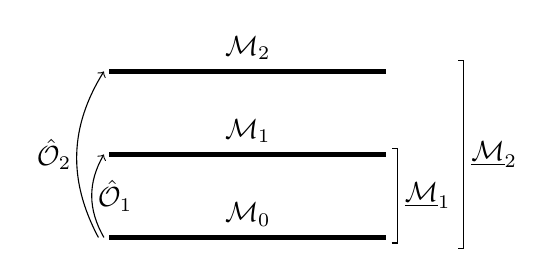
\begin{tikzpicture}
    \draw[ultra thick] (0,0) -- node[above] {$\M_0$} ++(10em,0);
    \draw[ultra thick] (0,3em) -- node[above] {$\M_1$} ++(10em,0);
    \draw[ultra thick] (0,2*3em) -- node[above] {$\M_2$} ++(10em,0);
    \draw[->] (-.2em,0) to [bend left] (-.2em,3em);
    \node (X) at (.2em,0.5*3em) {$\hat\O_1$};
    \draw[->] (-.4em,0) to [bend left] (-.2em,2*3em);
    \node (XY) at (-2em,3em) {$\hat\O_2$};
    \draw (10em+.2em,-.2em) -- (10em+.4em,-.2em)
    -- (10em+.4em,3em+.2em) -- (10em+.2em,3em+.2em);
    \node (cM1) at (10em+1.5em,0.5*3em) {$\col\M_1$};
    \draw (10em+2.4em+.2em,-.4em) -- (10em+2.4em+.4em,-.4em)
    -- (10em+2.4em+.4em,6em+.4em) -- (10em+2.4em+.2em,6em+.4em);
    \node (cM1) at (10em+2.4em+1.5em,3em) {$\col\M_2$};
  \end{tikzpicture}
  \caption{Schematic of low-lying multi-body manifolds.  Starting with
    the permutationally-state manifold $\M_0$, the single-body
    excitation manifold $\M_1$ consists of states accessible via
    single-body perturbations $\hat\O_1$.  The two-body excitation
    manifold $\hat\O_2$ then consists of states accessible via
    two-body perturbations, but not single-body perturbations.  The
    joint manifold $\col\M_M$ consists of all states accessible by
    operators $r$-body operators $\O_r$ with $r\le M$.}
  \label{fig:manifold_sketch}
\end{figure}

By construction, the $M$-body operator $X_{\m w}$ generally couples PS
states in $\M_0$ to asymmetric states in $\ul\M_M$.  If the coupling
between $\M_0$ and its complement is weak compared to the spectral gap
$\Delta_{\t{gap}}$ of $H_0$, then we can treat the effect of
$X_{\m w}$ perturbatively and derive an effective Hamiltonian
$H_{\t{eff}}$ on $\M_0$.  This ground-state perturbation theory
formally breaks down when the operator norm
$\norm{X_{\m w}}\ge\Delta_{\t{gap}}/2$, in which case the operator
$X_{\m w}$ first couples $\M_0$ to $\ul\M_M$, then $\ul\M_M$ to
$\ul\M_{2M}$, and so on.  Even if
$\norm{X_{\m w}}>\Delta_{\t{gap}}/2$, however, the energetic penalty
incurred by $H_0$ from breaking the permutational symmetry of an
initial state $\ket\psi\in\M_0$ suppresses the leakage of population
into manifolds $\M_r$ of increasing $r$.  One might therefore capture
the dynamics of an initial PS state $\ket\psi\in\M_0$ by projecting
$X_{\m w}$ onto $\ul\M_{r_{\t{max}}}$ for some $r_{\t{max}}\ge M$,
resulting in a theory that resembles first-order perturbation theory
on $\ul\M_{r_{\t{max}}}$.  In the perturbative regime
$\norm{X_{\m w}}<\Delta_{\t{gap}}/2$, such a theory captures all
virtual processes through order $2\floor{r_{\t{max}}/M}+1$ in a formal
perturbation theory on $\M_0$.  In the non-perturbative regime
$\norm{X_{\m w}}\ge\Delta_{\t{gap}}/2$, the error incurred by
truncating the Hilbert space of a spin system past
$\ul\M_{r_{\t{max}}}$ is not clear a priori.  Nonetheless, simulations
restricted to $\ul\M_{r_{\t{max}}}$ can be benchmarked by examining
the maximum populations within all $\M_r$ for $r\le r_{\t{max}}$
throughout simulation.  As long as
\begin{enumerate*}
\item these populations fall off with increasing $r$,
\item and the maximal population within large-$r$ manifolds $\M_r$ is
  small,
\end{enumerate*}
one should expect such simulations to faithfully capture (at least
qualitatively) the dynamical behavior of the spin system under
consideration.

In order to project an operator $X_{\m w}$ onto $\ul\M_{r_{\t{max}}}$,
we first need to construct a basis for $\ul\M_{r_{\t{max}}}$, and then
compute all matrix elements of $X_{\m w}$ in this basis.  Our strategy
will be to first identify a basis for $\M_0$, and then find, for each
$r=1,\cdots,r_{\t{max}}$, a suitable set of $r$-body operators
$\set{O}$ and dimension-$r$ tensors $\set{\m u}$ for which the states
$\ket{O,\m u,m}\propto O_{\m u}\ket{m}$ form an orthonormal basis for
$\M_r$.  Matrix elements of $X_{\m w}$ with respect to this basis for
$\ul\M_{r_{\t{max}}}$ then take the form
\begin{align}
  \bk{O,\m u,\ell|X_{\m w}|Q,\m v,m}
  = \f{\bk{\ell|O_{\m u}^\dag X_{\m w} Q_{\m v}|m}}
  {\sqrt{\bk{\ell|O_{\m u}^\dag O_{\m u}|\ell}
      \bk{m|Q_{\m v}^\dag Q_{\m v}|m}}}.
  \label{eq:matrix_element}
\end{align}
In order to compute these matrix elements, we simplify products of the
form $\P_0 O_{\m u}^\dag X_{\m w} Q_{\m v} \P_0$ and
$\P_0 O_{\m u}^\dag O_{\m u} \P_0$, with $\P_0$ a projector onto
$\M_0$, in Appendix \ref{sec:operator_product}.

Denoting all assignments of $N$ (identical) spins to $n$ (distinct)
states by $\A_n\p{N}$, a suitable basis for $\M_0$ is the set of PS
states $\set{\ket{m}:m\in\A_n\p{N}}$, where $m=\p{m_1,m_2,\cdots,m_n}$
specifies the occupation number $m_\mu$ of each single-spin state
$\mu$.  For consistency with the expression of matrix elements in
\eqref{eq:matrix_element}, for each $\ket{m}\in\M_0$ we define
$\ket{\1,1,m}\equiv\ket{m}$, with $\1$ the identity operator, and we
define $\1_1\equiv\1$.  We now need to determine the set of $r$-body
operators $\set{O}$ and dimension-$r$ tensors $\set{\m u}$ that define
our basis for each $\M_r$.  As an initial guess for $\set{\m u}$, we
can choose the set $\set{\m u_\Delta}_{\m h,r}$ of dimension-$r$
tensors $\m u_\Delta$ that generate eigenstates of $H_0$, i.e.~for
which $\hat{\m h}\p{\m u_\Delta} = \Delta \m u_\Delta$, with
$\hat{\m h}$ defined in \eqref{eq:multi_body_op}.  The set of $r$-body
operators to choose is less obvious, but can be determined by an
exhaustive search over all $r$-body operators relevant to a particular
scenario.  Specifically, the purpose of projecting operators onto
$\col\M_{r_{\t{max}}}$ is to simulate the dynamics induced by some
operator $\hat\O$ of the form in \eqref{eq:pert}, constructed from a
set $\O=\set{\p{X,\m w}}$ containing multi-spin operators $X$.  In
order to find a basis for the {\it relevant} states in $\M_r$, one can
simply consider the set $\set{O}_{\O,r}$ all $r$-spin operators that
can be constructed from products of the multi-spin operators $X$ in
$\O$.

In general, the states $\ket{O,\m u_\Delta,m}$ for all
$\p{O,\m u_\Delta,m}\in\set{O}_{\O,r}\times\set{\m u_\Delta}_{\m h,r}
\times\A_n\p{N}$ will form an overcomplete basis for the relevant
states in $\col\M_r$.  Our last step is therefore to reduce this set
of states to a minimal basis $\B_r$ for $\M_r$.  To this end, we
construct each of $\B_1,\B_2,\cdots,\B_{r_{\t{max}}}$ in sequence,
such that when constructing $\B_r$ we already have a minimal basis
$\col\B_{r-1}\equiv\bigcup_{s<r}\B_s$ for $\col\M_{r-1}$.  To
construct $\B_r$, we then consider each
$\p{O,\m u_\Delta,m}\in\set{O}_{\O,r}\times\set{\m u_\Delta}_{\m h,r}
\times\A_n\p{N}$ one at a time.  If $\ket{O,\m u_\Delta,m}$ is
orthogonal to all states in $\col\B_{r-1}$, as well as all other
states we have added to $\B_r$ thus far, then we include it in $\B_r$.
Otherwise, we discard $\ket{O,\m u_\Delta,m}$.  There are two
considerations to keep in mind for this construction: first, one
should always throw out null states $\ket{O,\m u_\Delta,m}=0$, which
can be identified by a vanishing self-overlap,
$\bk{O,\m u_\Delta,m|O,\m u_\Delta,m}=0$.  Second, computing overlaps
to check for orthogonality can be computationally intensive.  When
considering a candidate state $\ket{O,\m u_\Delta,m}$ to add to
$\B_r$, one can therefore restrict orthogonality checks to other
states $\ket{Q,\m v_\epsilon,\ell}$ with $\epsilon=\Delta$; if the
excitation energies $\epsilon\ne\Delta$, then these states are
guaranteed to be orthogonal.  Any two states with different occupation
numbers of single-spin states $\mu\in\ZZ_n$ are similarly guaranteed
to be orthogonal.

%%%%%%%%%%%%%%%%%%%%%%%%%%%%%%%%%%%%%%%%%%%%%%%%%%%%%%%%%%%%%%%%%%%%%%
\section{The XXZ model}


\red{[TODO: write section]}



\newpage
\appendix

%%%%%%%%%%%%%%%%%%%%%%%%%%%%%%%%%%%%%%%%%%%%%%%%%%%%%%%%%%%%%%%%%%%%%%
\section{Existence of a spectral gap with long-range power-law
  interactions}
\label{sec:spectral_gap}

Here we show that power-law SU($n$)-symmetric interactions of the form
in \eqref{eq:H_0} with $h_{pq}=-h/\abs{p-q}^\alpha$ yield a
non-vanishing many-body interaction energy gap when $\alpha\le D$,
where $D$ is the dimension of the lattice.  On a periodic lattice of
$N=L^D$ spins, the spectral gap of the interaction Hamiltonian is (see
Appendix \ref{sec:single_body_eigenstates})
\begin{align}
  \Delta
  = \sum_{d\in\ZZ_L^D} h_{0,d} \sp{\cos\p{d \c k_{\t{SE}}}-1}
  = h \sum_{\substack{d\in\ZZ_L^D\\\abs{d}\ge1}}
  \f{1-\cos\p{d \c k_{\t{SE}}}}{\abs{d}^\alpha},
\end{align}
where $\ZZ_L$ denotes the integers modulo $L$;
$k_{\t{SE}}\in\ZZ_L^D\times2\pi/L$ is a wavenumber for a
singly-excited spin-wave state; and the norm $\abs{d}$ for a vector
$d$ on a periodic lattice is implicitly understood to mean the
smallest Euclidean distance of $d$ from a fixed origin.  In order to
yield the smallest excitation energy $\Delta$, the wavenumber
$k_{\t{SE}}$ should maximize the contribution of the cosine term
above, which is achieved by a wavenumber that minimizes the
oscillations of this term when integrated over the entire lattice.  A
suitable candidate for a minimal wavenumber is
$k_{\t{SE}}=\p{2\pi/L,0,0,\cdots}$, which corresponds to an excitation
energy
\begin{align}
  \Delta = h \sum_{\substack{d\in\ZZ_L^D\\\abs{d}\ge1}}
  \f{1-\cos\p{d_12\pi/L}}{\abs{d}^\alpha}.
\end{align}
Defining $\epsilon\equiv2/L$ and a rescaled domain symmetrized about
$0$, $\SS_\epsilon\simeq\ZZ_L/\epsilon$ with
$\SS_\epsilon\subset\sp{-1,1}$, we substitute $x\simeq\epsilon d$ to
get
\begin{align}
  \Delta
  = h \sum_{\substack{x\in\SS_\epsilon^D\\\abs{x}\ge\epsilon}}
  \f{1-\cos\p{\pi x_1}}{\abs{x/\epsilon}^\alpha}
  = h \epsilon^{\alpha-D} \sum_{\substack{x\in\SS_L^D\\\abs{x}\ge\epsilon}}
  \epsilon^D \f{1-\cos\p{\pi x_1}}{\abs{x}^\alpha}.
\end{align}
As $\epsilon\to0$ the discrete sum over $x$ is well approximated by an
integral that avoids an infinitesimal region about the origin, i.e.
\begin{align}
  \Delta = h \epsilon^{\alpha-D} \I_{D\epsilon},
  &&
  \I_{D\epsilon}
  \equiv \int_{\TT_1^D\setminus\TT_\epsilon^D} \d^Dx\,
  \f{1-\cos\p{\pi x_1}}{\abs{x}^\alpha},
\end{align}
where the integral $\I_{D\epsilon}$ is defined using the interval
$\TT_a\equiv\p{-a,a}$.  The integrand of $\I_{D\epsilon}$ is strictly
positive and well-behaved on the entirety of its domain except for the
origin, where depending on the value of $\alpha$ the integrand may
vanish or diverge as $\abs{x}\to0$.  Together, these facts mean that
\begin{align}
  \I_{D\epsilon} \stackrel{\epsilon\to0}{\sim} \epsilon^{-\gamma},
  &&
  \Delta \stackrel{\epsilon\to0}{\sim} h \epsilon^{\alpha-D-\gamma},
\end{align}
for some $\gamma\ge0$, which implies that gap $\Delta$ is
non-vanishing when $\alpha\le D\le D+\gamma$.

For the sake of completion, we add that in fact the gap $\Delta$
always vanishes in the thermodynamic limit when $\alpha>D$.  To see
this behavior, we note that the asymptotic dependence of the integral
$\I_{D\epsilon}$ on $\epsilon$ is determined by the behavior of its
integrand when $\abs{x}\sim\epsilon$, in which case
$1-\cos\p{\pi x_1}\sim x_1^2$, so
\begin{align}
  \I_{D\epsilon}
  \sim \int_{\TT_1^D\setminus\TT_\epsilon^D} \d^Dx\,
  \f{x_1^2}{\abs{x}^\alpha}.
\end{align}
We can then use the fact that $x_1^2\le\abs{x}^2$ and change to
spherical coordinates to find that
\begin{align}
  \I_{D\epsilon} \lesssim
  \int_{\TT_1^D\setminus\TT_\epsilon^D} \d^Dx\,
  \f{\abs{x}^2}{\abs{x}^\alpha}
  \sim \int_\epsilon^1 \d x\, x^{D+1-\alpha}
  \sim
  \begin{cases}
    \epsilon^0 & \alpha < D+2 \\
    \log\p{1/\epsilon} & \alpha = D+2 \\
    \epsilon^{D+2-\alpha} & \alpha > D+2
  \end{cases}.
\end{align}
It follows that the spectral gap
\begin{align}
  \Delta \stackrel{\epsilon\to0}{\lesssim}
  \begin{cases}
    \epsilon^{\alpha-D} & \alpha < D+2 \\
    \epsilon^2 \log\p{1/\epsilon} & \alpha = D + 2 \\
    \epsilon^2 & \alpha > D+2
  \end{cases},
\end{align}
which vanishes as $\epsilon\to0$ for all $\alpha>D$.

%%%%%%%%%%%%%%%%%%%%%%%%%%%%%%%%%%%%%%%%%%%%%%%%%%%%%%%%%%%%%%%%%%%%%%
\section{Constructing excitation energy eigenstates}
\label{sec:eigenstates}

In this section, we simplify the products of the form
$H_0X_{\m w}\ket\psi$ to find conditions under which a multi-body
perturbation $X_{\m w}$ generates eigenstates of the SU($n$)-symmetric
interaction Hamiltonian $H_0$ in \eqref{eq:H_0} when acting on a
permutationally symmetric state $\ket\psi\in\M_0$.  Here $X_{\m w}$ is
an $M$-body perturbation defined by
\begin{align}
  X_{\m w}
  \equiv \f1{M!} \sum_{k\in\D_N\p{M}} w_k X_k,
\end{align}
where $X$ is an $M$-spin operator; $k\equiv\p{k_1,k_2,\cdots,k_M}$ is
a list of $M$ spins that $X_k$ acts on; $\m w$ is a dimension-$M$
(i.e.~$M$-index) tensor with scalar entries $w_k$; and $\D_N\p{M}$ is
the strictly off-diagonal part of $\ZZ_N^M$, defined in
\eqref{eq:off_diags}.

%%%%%%%%%%%%%%%%%%%%%%%%%%%%%%%%%%%%%%%%%%%%%%%%%%
\subsection{Single-body excitations}
\label{sec:single_body_eigenstates}

In order to build familiarity with the problem at hand, we first
consider the simple case of a single-body perturbation and simplify
\begin{align}
  H_0 X_{\m w} \ket\psi
  = \sum_{\substack{k\in\ZZ_N\\\set{p,q}\in\C_N\p{2}}}
  h_{pq} w_k \Pi_{pq} X_k \ket\psi.
  \label{eq:single_body_diagnosis_start}
\end{align}
The sum in \eqref{eq:single_body_diagnosis_start} has terms with
$k\notin\set{p,q}$, and terms with $k\in\set{p,q}$.  In the case of
$k\notin\set{p,q}$, the permutation operator $\Pi_{pq}$ commutes with
$X_k$ and annihilates on $\ket\psi$, allowing us to simplify
\begin{align}
  \sum_{k\in\ZZ_N} \sum_{\substack{\set{p,q}\in\C_N\p{2}\\k\notin\set{p,q}}}
  h_{pq} w_k \Pi_{pq} X_k \ket\psi
  = E_0 X_{\m w} \ket\psi
  - \sum_{k\in\ZZ_N} \sum_{\substack{\set{p,q}\in\C_N\p{2}\\k\in\set{p,q}}}
  h_{pq} w_k X_k \ket\psi,
\end{align}
where $E_0 = \sum_{\set{p,q}\in\C_N\p{2}} h_{pq}$ is the interaction
energy of PS states $\ket\psi\in\M_0$, and
\begin{align}
  \sum_{\substack{\set{p,q}\in\C_N\p{2}\\k\in\set{p,q}}} h_{pq}
  = \f12 \sum_{\substack{p,q\in\ZZ_N\\k\in\set{p,q}}} h_{pq}
  = \f12 \sum_{p\in\ZZ_N} h_{pk} + \f12 \sum_{q\in\ZZ_N} h_{kq}
  = h_k,
  &&
  h_k \equiv \sum_{p\in\ZZ_N} h_{pk},
\end{align}
which implies
\begin{align}
  \sum_{k\in\ZZ_N} \sum_{\substack{\set{p,q}\in\C_N\p{2}\\k\notin\set{p,q}}}
  h_{pq} w_k X_k \ket\psi
  = E_0 X_{\m w} \ket\psi
  - \sum_{k\in\ZZ_N} h_k w_k X_k \ket\psi.
\end{align}
The terms in \eqref{eq:single_body_diagnosis_start} with
$k\in\set{p,q}$, meanwhile, are
\begin{align}
  \sum_{\substack{\set{p,q}\in\C_N\p{2}\\k\in\set{p,q}}}
  h_{pq} w_k \Pi_{pq} X_k \ket\psi
  = \sum_{k,q\in\ZZ_N} h_{kq} w_k X_q \ket\psi,
\end{align}
so in total
\begin{align}
  H_0 X_{\m w} \ket\psi
  = E_0 X_{\m w} \ket\psi
  + \sum_{p\in\ZZ_N} \p{\sum_{q\in\ZZ_N} h_{pq} w_q - h_p w_p}
  X_p \ket\psi.
  \label{eq:single_body_diagnosis_end}
\end{align}
The action of the single-body perturbation $X_{\m w}$ on a
permutationally symmetric state therefore generates an eigenstate of
$H_0$ with energy $E_0+\Delta$ if the vector
$\v{\m w}\equiv\sum_{k\in\ZZ_N} w_k \ket{k}$ satisfies the eigenvalue
equation
\begin{align}
  \p{\m h - \diag\v h} \c \v{\m w} = \Delta \v{\m w},
  \label{eq:single_body_eig}
\end{align}
where $\m h\equiv\sum_{p,q\in\ZZ_N} h_{pq} \op{p}{q}$ is a matrix of
all couplings $h_{pq}$; the vector
$\v h \equiv \sum_{p\in\ZZ_N} h_p \ket{p} = \sum_{p,q\in\ZZ_N} h_{pq}
\ket{p}$ is the sum of all columns of $\m h$; and $\diag\v h$ is a
matrix with $\v h$ on the diagonal and zeroes everywhere else.

When the interaction Hamiltonian $H_0$ is translationally invariant,
the single-body eigenvalue problem in \eqref{eq:single_body_eig} is
solvable analytically.  In this case, the couplings $h_{pq}$ depend
only on the separation $\abs{p-q}$, so eigenvectors of $\m h$ are
therefore plane waves of the form
\begin{align}
  \v{\m w}_k \equiv \sum_{p\in\ZZ_L^D} e^{ip\c k} \ket{p},
\end{align}
where on a $D$-dimensional periodic lattice of $N=L^D$ spins, lattice
sites are indexed by vectors $p\in\ZZ_L^D$, and wavenumbers take on
values $k\in\ZZ_L^D\times2\pi/L$.  The corresponding eigenvalues of
$\m h$ can be determined by expanding
\begin{align}
  \m h\c{\m w}_k
  = \sum_{p,q\in\ZZ_L^D} h_{pq} e^{iq\c k} \ket{p}
  = \sum_{p,d\in\ZZ_L^D} h_{p,p+d} e^{i\p{p+d}\c k} \ket{p}
  = \sum_{d\in\ZZ_L^D} h_{0,d} \cos\p{d\c k} \v{\m w}_k,
\end{align}
where the imaginary contributions vanish because $h_{0,d}=h_{0,-d}$.
The remainder of \eqref{eq:single_body_eig} that we need to sort out
is $\diag\v h$, where all
$h_p=\sum_{q\in\ZZ_L^D}h_{pq}=\sum_{d\in\ZZ_L^D}h_{0,d}$ are equal,
which implies that $\diag\v h=\sum_{d\in\ZZ_L^D}h_{0,d}$ is a scalar.
We thus find that
\begin{align}
  \p{\m h - \diag\v h}\c\v{\m w}_k = \Delta_k \v{\m w}_k,
  &&
  \Delta_k \equiv \sum_{d\in\ZZ_L^D} h_{0,d} \sp{\cos\p{d\c k}-1}.
\end{align}

%%%%%%%%%%%%%%%%%%%%%%%%%%%%%%%%%%%%%%%%%%%%%%%%%%
\subsection{Multi-body excitations}

We now consider the full $M$-body case
\begin{align}
  H_0 \tilde X_{\m w} \ket\psi
  = \sum_{\substack{k\in\D_N\p{M}\\\set{p,q}\in\C_N\p{2}}}
  h_{pq} w_k \Pi_{pq} X_k \ket\psi,
  \label{eq:diagnosis_start}
\end{align}
where to avoid factors of $M!$ in this section, we define
$\tilde X_{\m w}\equiv M! X_{\m w}$.  The sum in
\eqref{eq:diagnosis_start} has terms with $p,q\notin k$, terms with
$p,q\in k$, and terms with only one of $p$ or $q\in k$.  The
permutation operator $\Pi_{pq}$ acts trivially on $X_k\ket\psi$ when
$p,q\notin k$, allowing us to simplify
\begin{align}
  \sum_{\substack{k\in\D_N\p{M}\\\set{p,q}\in\C_N\p{2}\\p,q\notin k}}
  h_{pq} w_k \Pi_{pq} X_k \ket\psi
  = E_0 \tilde X_{\m w} \ket\psi
  - \sum_{k\in\D_N\p{M}} h^{\t{D}}_k w_k X_k \ket\psi,
\end{align}
where $E_0 = \sum_{\set{p,q}\in\C_N\p{2}} h_{pq}$ is the interaction
energy of PS states $\ket\psi\in\M_0$, and
\begin{align}
  h^{\t{D}}_k \equiv
  \sum_{\substack{\set{p,q}\in\C_N\p{2}\\p\in k~\t{or}~q\in k}} h_{pq}
  = \sum_{p\in k} h_p - \sum_{\set{a,b}\in\C_M\p{2}} h_{k_ak_b},
  &&
  h_p \equiv \sum_{q\in\ZZ_N} h_{pq}.
  \label{eq:multi_body_op_diag_element}
\end{align}
Defining a linear operator $\m h_{\t{D}}$ on the space of
dimension-$M$ tensors, whose action on $\m w$ is a new dimension-$M$
tensor with entries
\begin{align}
  \m h_{\t{D}}\p{\m w}_k \equiv h^{\t{D}}_k w_k,
  \label{eq:multi_body_op_diag}
\end{align}
we can write the terms in \eqref{eq:diagnosis_start} with
$p,q\notin k$ as
\begin{align}
  \sum_{\substack{k\in\D_N\p{M}\\\set{p,q}\in\C_N\p{2}\\p,q\notin k}}
  h_{pq} w_k \Pi_{pq} X_k \ket\psi
  = E_0 \tilde X_{\m w} \ket\psi
  - \sum_{k\in\D_N\p{M}} \m h_{\t{D}}\p{\m w}_k X_k \ket\psi.
\end{align}
The terms in \eqref{eq:diagnosis_start} with $p,q\in k$ are
\begin{align}
  \sum_{\substack{k\in\D_N\p{M}\\\set{p,q}\in\C_N\p{2}\\p,q\in k}}
  h_{pq} w_k \Pi_{pq} X_k \ket\psi
  = \sum_{k\in\D_N\p{M}} \sum_{\substack{\set{a,b}\in\C_M\p{2}}}
  h_{k_ak_b} w_{k_{a\lra b}} X_k \ket\psi,
\end{align}
where $k_{a\lra b}$ denotes a list that is equal to
$k=\p{k_1,k_2,\cdots,k_M}$ but with $k_a$ and $k_b$ swapped, and we
have relabeled $k_a$ and $k_b$ to change $w_k X_{k_{a\lra b}}$ to
$w_{k_{a\lra b}} X_k$.  To write down these terms succinctly, we
define a linear operator $\m h_{\t{P}}$ on the space of dimension-$M$
tensors, whose action on $\m w$ is a new dimension-$M$ tensor with
entries
\begin{align}
  \m h_{\t{P}}\p{\m w}_k
  \equiv \sum_{\substack{\set{a,b}\in\C_M\p{2}}}
  h_{k_ak_b} w_{k_{a\lra b}},
  \label{eq:multi_body_op_perm}
\end{align}
such that
\begin{align}
  \sum_{\substack{k\in\D_N\p{M}\\\set{p,q}\in\C_N\p{2}\\p,q\in k}}
  h_{pq} w_k \Pi_{pq} X_k \ket\psi
  = \sum_{k\in\D_N\p{M}} \m h_{\t{P}}\p{\m w}_k X_k \ket\psi.
\end{align}
Finally, the terms in \eqref{eq:diagnosis_start} with only one of
$p\in k$ or $q\in k$ are
\begin{align}
  \sum_{k\in\D_N\p{M}} \sum_{\substack{p\in\ZZ_N\\p\notin k}}
  \sum_{q\in k} h_{pq} w_k  \Pi_{pq} X_k \ket\psi
  = \sum_{k\in\D_N\p{M}} \sum_{\substack{p\in\ZZ_N\\p\notin k}}
  \sum_{a\in\ZZ_M} h_{pk_a} w_{k_{a:p}} X_k \ket\psi,
\end{align}
where $k_{a:p}$ denotes a list that is equal to $k$ but with $k_a$
replaced by $p$, and we have relabeled $k_a$ and $p$ to change
$w_k X_{k_{a:p}}$ to $w_{k_{a:p}} X_k$.  For each fixed $a$, the sum
over $p$ above is essentially a contraction of the matrix $\m h$ with
the $a$-th index of the tensor $\m w$.  Defining a linear operator
$\m h_a$ on the space of dimension-$M$ tensors, whose action on $\m w$
is a new dimension-$M$ tensor with entries
\begin{align}
  \m h_a\p{\m w}_k
  \equiv \sum_{\substack{p\in\ZZ_N\\p\notin k}} h_{pk_a} w_{k_{a:p}}
  = \sum_{\substack{p\in\ZZ_N\\p\notin k}}
  h_{pk_a} w_{k_1 k_2 \cdots k_{a-1} p k_{a+1} \cdots k_M},
  \label{eq:multi_body_op_contract}
\end{align}
we can expand
\begin{align}
  \sum_{k\in\D_N\p{M}} \sum_{\substack{p\in\ZZ_N\\p\notin k}}
  \sum_{q\in k} h_{pq} w_k  \Pi_{pq} X_k \ket\psi
  = \sum_{k\in\D_N\p{M}} \sum_{a\in\ZZ_M}
  \m h_a\p{\m w}_k X_k \ket\psi.
\end{align}
Altogether, we find that
\begin{align}
  H_0 X_{\m w} \ket\psi
  = E_0 X_{\m w} \ket\psi + X_{\hat{\m h}\p{\m w}} \ket\psi,
\end{align}
where
\begin{align}
  \hat{\m h}\p{\m w}
  \equiv \sum_{a\in\ZZ_M} \m h_a\p{\m w}
  + \m h_{\t{P}}\p{\m w} - \m h_{\t{D}}\p{\m w},
\end{align}
is defined in terms of the tensors $\m h_a\p{\m w}$,
$\m h_{\t{P}}\p{\m w}$, and $\m h_{\t{D}}\p{\m w}$, whose entries are
respectively provided in \eqref{eq:multi_body_op_contract},
\eqref{eq:multi_body_op_perm}, and \eqref{eq:multi_body_op_diag}.  The
action of the $M$-body perturbation $X_{\m w}$ on a permutationally
symmetric state therefore generates an eigenstate of $H_0$ with energy
$E_0+\Delta$ if the coefficient tensor $\m w$ satisfies the
generalized eigenvalue equation $\hat{\m h}\p{\m w} = \Delta \m w$,
which can be written in the form
\begin{align}
  \hat{\m h} \c \v{\m w} = \Delta \v{\m w},
  &&
  \v{\m w} \equiv \sum_{k\in\D_N\p{M}} w_k \ket{k},
  \label{eq:multi_body_problem}
\end{align}
where
\begin{align}
  \hat{\m h} \equiv \sum_{k\in\D_N\p{M}} \ket{k}
  \sp{\sum_{a\in\ZZ_M} \sum_{\substack{p\in\ZZ_N\\p\notin k}}
    h_{pk_a} \bra{k_{a:p}}
    + \sum_{\set{a,b}\in\C_M\p{2}} h_{k_ak_b} \bra{k_{a\lra b}}
    - h^{\t{D}}_k \bra{k}}.
  \label{eq:multi_body_mat}
\end{align}
If the coefficient tensor $\m w$ is permutationally symmetric, meaning
that $\m w$ is invariant under arbitrary permutations of its tensor
factors, then this symmetry is preserved by $\hat{\m h}$.  In this
case, we can replace sums over $k\in\D_N\p{M}$ in
\eqref{eq:multi_body_problem} and \eqref{eq:multi_body_mat} by sums
over $k\in\C_N\p{M}$, and replace vectors
$\ket{\p{k_1,k_2,\cdots,k_M}}\to\ket{\set{k_1,k_2,\cdots,k_M}}$, such
that e.g.~$\ket{k_{a\lra b}}=\ket{k}$.  These replacements reduce the
size of $\hat{\m h}$ from $N!_M\times N!_M$ to
${N\choose M}\times{N\choose M}$, where
$N!_M=M!\times{N\choose M}=\prod_{j=0}^{M-1}\p{N-j}$ denotes a falling
factorial.  We discuss further reduction of the eigenvalue problem in
\eqref{eq:multi_body_problem} by use of additional symmetries in
Section \ref{sec:symmetries}.

Some special cases: if $M=1$, then $h^{\t{D}}_k=h_k$, so
\begin{align}
  \hat{\m h} \stackrel{M=1}{=} \sum_{k\in\ZZ_N} \ket{k}
  \sp{\sum_{\substack{p\in\ZZ_N\\p\ne k}} h_{pk} \bra{p} - h_k \bra{k}}
  = \m h - \diag\v h,
\end{align}
which is precisely what we found in \eqref{eq:single_body_eig}.  If
$M=2$, then $h_{k\ell}^{\t{D}}=h_k+h_\ell-h_{k\ell}$, so
\begin{align}
  \hat{\m h} \stackrel{M=2}{=}
  \sum_{\p{k,\ell}\in\D_N\p{2}} \ket{k,\ell}
  \sp{\sum_{\substack{p\in\ZZ_N\\p\notin\set{k,\ell}}}
    \p{ h_{pk} \bra{p,\ell} + h_{p\ell} \bra{k,p} }
    + h_{k\ell} \bra{\ell,k}
    - \p{h_k + h_\ell - h_{k\ell}} \bra{k,\ell}}.
\end{align}

%%%%%%%%%%%%%%%%%%%%%%%%%%%%%%%%%%%%%%%%%%%%%%%%%%
\subsection{Exploiting spatial symmetries}
\label{sec:symmetries}

Solving the eigenvalue problem in \eqref{eq:multi_body_problem} to
find $M$-body operators $X_{\m w}$ that generate states of definite
interaction energy nominally requires diagonalizing the matrix
$\hat{\m h}$ with dimensions $N!_M\times N!_M\sim N^M\times N^M$,
where $N!_M=\prod_{j=0}^{M-1}\p{N-j}$ denotes a falling factorial.
Spatial symmetries of the interaction Hamiltonian $H_0$, however,
generally endow $\hat{\m h}$ with a block-diagonal structure that can
be used to reduce the complexity of this eigenvalue problem.
Translational invariance, for example, can reduce this problem to that
of diagonalizing a matrix with dimensions
$\sim N^{M-1}\times N^{M-1}$, and isotropy can further reduce the
problem size by factors that depend on the lattice geometry.  The
complexity of diagonalizing a matrix with dimensions $d\times d$ is
$O\p{d^3}$, so even a reduction of $d$ by a factor of 2 yields
practically significant gains (a factor of $2^3=8$) in the runtime of
diagonalization.  Here, we provide a general prescription for
exploiting the spatial symmetries of $H_0$ to simplify the eigenvalue
problem in \eqref{eq:multi_body_problem}.

Our task is essentially to express the multi-body eigenvalue problem
in \eqref{eq:multi_body_problem} in a basis that respects the spatial
symmetries of $H_0$.  These symmetries essentially break the set
$\D_N\p{M}$ into equivalence classes $\S_M$\footnote{For brevity, we
  will suppress the explicit dependence of $\S_M$ on $N$, as well as
  the dependence of $\S_M$ on any other factors such as lattice
  geometry.}, where elements $s\in\S_M$ are subsets
$s\subset\D_N\p{M}$ that are invariant under the appropriate symmetry
group action.  In the case of $M=2$ in a translationally invariant and
isotropic system, for example, each equivalence class $s\in\S_2$ would
consist of all pairs $\p{p,q}\in\D_N\p{2}$ that are a fixed distance
$\abs{p-q}=d_s$ apart,
i.e.~$s=\set{\p{p,q}\in\D_N\p{2}:\abs{p-q}=d_s}$.  If the tensor
$\m w$ is invariant under arbitrary permutations of its tensor
factors, this symmetry is preserved by $\hat{\m h}$, and we can place
all $k\in\D_N\p{M}$ that are equal up to permutation into the same
equivalence class.

For simplicity, we first assume that the $M$-body operator $X_{\m w}$
obeys the same spatial symmetries as $H_0$.  For any equivalence class
$s\in\S_M$, we then define a uniform superposition $\ket{s}$ over all
$k\in s$, as well as a projector $\P_\S$ onto the space of uniform
superpositions:
\begin{align}
  \ket{s} \equiv \f1{\sqrt{\abs{s}}} \sum_{k\in s} \ket{k},
  &&
  \P_{\S_M} \equiv \sum_{s\in\S_M} \op{s},
\end{align}
where $\abs{s}$ is the number of elements in $s$.  In turn, we expand
the coefficient vector $\v{\m w}$ in this symmetrized basis:
\begin{align}
  \v{\m w} = \P_{\S_M} \v{\m w}
  = \sum_{s\in\S_M} \sum_{k\in s} w_k \ket{s} \bk{s|k}
  = \sum_{s\in\S_M} w_s \sqrt{\abs{s}} \ket{s},
\end{align}
where all $w_k$ with $k\in s$ are equal by assumption, so we can
define $w_s\equiv w_k$ for any $k\in s$.  Finally, we expand the
projection of $\hat{\m h}$ onto the symmetric subspace:
\begin{align}
  \P_{\S_M} \hat{\m h} \P_{\S_M}
  = \sum_{s\in\S_M} \f{\ket{s}}{\sqrt{\abs{s}}} \sp{
    \sum_{\substack{k\in s\\a\in\ZZ_M}}
    \sum_{\substack{p\in\ZZ_N\\p\notin k}}
    h_{p k_a} \f{\bra{\sp{k_{a:p}}}}{\sqrt{\abs{\sp{k_{a:p}}}}}
    + \sum_{\set{a,b}\in\C_M\p{2}} h_{k_ak_b}
    \f{\bra{\sp{k_{a\lra b}}}}{\sqrt{\abs{\sp{k_{a\lra b}}}}}
    - h^{\t{D}}_s \f{\bra{s}}{\sqrt{\abs{s}}}},
\end{align}
where $h^{\t{D}}_s\equiv h^{\t{D}}_k$ for any $k\in s$, with
$h^{\t{D}}_k$ defined in \eqref{eq:multi_body_op_diag_element}; and
$\sp{k}$ denotes the equivalence class of $k$.  The reduced multi-body
eigenvalue problem is then
\begin{align}
  \P_{\S_M} \hat{\m h} \P_{\S_M} \c \v{\m w} = \Delta \v{\m w}.
\end{align}
More generally, even if the couplings $\v{\m w}$ of $X_{\m w}$ do not
obey the spatial symmetries as $H_0$, these symmetries generally endow
$\hat{\m h}$ with a block-diagonal structure that reduces the
complexity of the multi-body eigenvalue problem.  We leave this
reduction to future work.  % todo: perform reduction

%%%%%%%%%%%%%%%%%%%%%%%%%%%%%%%%%%%%%%%%%%%%%%%%%%%%%%%%%%%%%%%%%%%%%%
\section{Permutation-symmetrized products of multi-body operators}
\label{sec:operator_product}

\red{[TODO: write introductory text for this section]}

%%%%%%%%%%%%%%%%%%%%%%%%%%%%%%%%%%%%%%%%%%%%%%%%%%
\subsection{The general case: a diagrammatic expansion}

Given a system of $N$ spins, we wish to project a product of
multi-body operators onto the permutationally symmetric (PS) manifold
$\M_0$.  For $p$ multi-body operators, such a product takes the form
\begin{align}
  \m X_{\m w}
  \equiv \prod_{\alpha\in\ZZ_p} \f1{M_\alpha!}
  \sum_{k_\alpha\in\D_N\p{M_\alpha}}
  w_\alpha\p{k_\alpha} X_\alpha\p{k_\alpha}
  = \f1{\m M!} \sum_{k\in\D_N\p{\m M}} \prod_{\alpha\in\ZZ_p}
  w_\alpha\p{k_\alpha} X_\alpha\p{k_\alpha},
  \label{eq:sym_prod_start}
\end{align}
where $\m X\equiv\p{X_1,X_2,\cdots,X_p}$ is a vector of
$M_\alpha$-spin operators $X_\alpha$;
$\m w\equiv\p{w_1,w_2,\cdots,w_p}$ is a vector of dimension-$M_\alpha$
tensors $w_\alpha$; $\m M\equiv\p{M_1,M_2,\cdots,M_p}$ is a vector of
the dimensions $M_\alpha$;
$k_\alpha=\p{k_{\alpha,1},k_{\alpha,2},\cdots,k_{\alpha,M_\alpha}}$ is
a choice of $M_\alpha$ spins that $X_\alpha\p{k_\alpha}$ acts on;
$w_\alpha\p{k_\alpha}$ is a scalar entry of $w_\alpha$;
$\D_N\p{M_\alpha}$ is the strictly off-diagonal part of $\ZZ_N^M$,
defined in \eqref{eq:off_diags};
$\D_N\p{\m M}\equiv\bigotimes_{M_\alpha\in\m M}\D_N\p{M_\alpha}$, such
that each $k\in\D_N\p{\m M}$ has the decomposition
$k=\p{k_1,k_2,\cdots,k_p}$ with $k_\alpha\in\D_N\p{M_\alpha}$; and
$\m M!\equiv\prod_{M_\alpha\in\m M}M_\alpha!$ for shorthand.  For
later convenience, we define
$w_\alpha\p{k_\alpha}=X_\alpha\p{k_\alpha}=0$ for any $k_\alpha$ with
repeated entries.

We now classify terms in \eqref{eq:sym_prod_start} by the numbers
$g_S$ of indices shared by all tensors $w_\alpha$ with
$\alpha\in S\subset\ZZ_p$.  For example, a term of the form
$w_1\p{a,b,c} w_2\p{b,d,e} w_3\p{b,c,d,e}$ with distinct indices
$a,b,c,d,e$ would have
\begin{align}
  g_{\set{1}} = 1,
  &&
  g_{\set{1,2,3}} = 1,
  &&
  g_{\set{1,3}} = 1,
  &&
  g_{\set{2,3}} = 2,
\end{align}
and $g_S=0$ for all other subsets $S\subset\ZZ_3$.  This index
assignment can be associated with the Venn diagram
\begin{align}
  \diagram{example_123},
  \label{eq:venn_diagram}
\end{align}
where $g_S$ is determined the number of dots at the intersection of
circles $\alpha\in S$.  We denote the set of all nonempty subsets of
$\ZZ_p$ by $\PP^*\p{\ZZ_p}$, and denote a choice of $g_S$ for all
$S\in\PP^*\p{\ZZ_p}$ by $g$.  With representations such as
\eqref{eq:venn_diagram} in mind, we will loosely refer to $g$ as
simply a ``diagram''.  We define
$\abs{g}\equiv\sum_{S\in\PP^*\p{\ZZ_p}}g_S$ to be the number of
indices considered in $g$ (or equivalently the number of dots in the
diagram $g$), and we denote the set of all diagrams for
$p=\dim\p{\m M}$ tensors with dimensions $\m M$ by $\G\p{\m M}$.  For
consistency, all diagrams $g\in\G\p{\m M}$ must associate exactly
$M_\alpha$ indices with the dimension-$M_\alpha$ tensor $w_\alpha$,
i.e.
\begin{align}
  \sum_{S\in\PP^*\p{\ZZ_p}\,:\,\alpha\in S} g_S
  = \sum_{R\in\PP^*\p{\ZZ_p\setminus\set{\alpha}}} g_{\set{\alpha}\cup R}
  = M_\alpha
\end{align}
for all $\alpha\in\ZZ_p$.  A classification of the terms in
\eqref{eq:sym_prod_start} by diagrams $g\in\G\p{\m M}$ allows us to
expand
\begin{align}
  \m X_{\m w} \EQPS \sum_{g\in\G\p{\m M}} \m X_{\m w}\p{g},
  \label{eq:sym_prod_diagrams}
\end{align}
where $\EQPS$ denotes equality under a restriction to $\M_0$, and
$\m X_{\m w}\p{g}$ is the sum of all terms in
\eqref{eq:sym_prod_start} that are associated with the diagram $g$.

To find an explicit form of $\m X_{\m w}\p{g}$, we first consider all
distinct ways to assign $\abs{g}$ indices to specific tensor factors
of $\m w$ and $\m X$ in a manner consistent with $g$.  For example, if
$\m X=\p{X_1,X_2}$ with dimensions $\p{M_1,M_2}=\p{2,1}$ and
$\abs{g}=2$ with $g_{\set{1}}=g_{\set{1,2}}=1$, then
$X_1\p{a,b} X_2\p{b}$ and $X_1\p{b,a} X_2\p{b}$ are distinct
assignments of $\abs{g}$ indices to $\m X$ in a manner consistent with
$g$, provided that $a\ne b$.  After assigning $\abs{g}$ indices to
$\m w$ and $\m X$ in a manner consistent with $g$, we need to sum over
all values that these indices can take, which amounts to a sum over
all $k\in\D_N\p{\abs{g}}$.

A specific assignment of indices can be thought of as a choice, for
each of the $M_\alpha$ tensor factors of $w_\alpha$ and $X_\alpha$, of
which dot in the diagram $g$ that tensor factor is associated with
(i.e.~out of the $M_\alpha$ dots within circle $\alpha$).  There are
nominally $M_\alpha!$ such choices for a given $\alpha$, and therefore
$\prod_{\alpha\in\ZZ_p}M_\alpha!=\m M!$ choices total.  The only catch
is that these choices treat all dots in $g$ as distinct, whereas the
$g_S$ dots within region $S$ of $g$ are actually indistinguishable.
The assignment $X_1\p{a,b,c} X_2\p{a,b}$, for example, is the same as
$X_1\p{b,a,c} X_2\p{b,a}$, because $a$ and $b$ are dummy indices.
Treating $g_S$ dummy indices as as distinguishable results in
over-counting distinct index assignments by a factor of $g_S!$.
Denoting the set of all distinct index assignments according to $g$ by
$\L\p{g}$, the number of such assignments is therefore
\begin{align}
  \abs{\L\p{g}} = \m M! \times \S\p{g},
  &&
  \S\p{g} \equiv \sp{\prod_{S\in\PP^*\p{\ZZ_p}} g_S!}^{-1}.
  \label{eq:assignment_num}
\end{align}
Altogether, we have
\begin{align}
  \m X_{\m w}\p{g} \equiv \f{\S\p{g}}{\abs{\L\p{g}}}
  \sum_{\ell\in\L\p{g}} \sum_{k\in\D_N\p{\abs{g}}}
  \m w\p{k,\ell} \m X\p{k,\ell},
\end{align}
where $\m w\p{k,\ell}$ and $\m X\p{k,\ell}$ denote the scalar and
operator acquired by assigning the indices
$k=\p{k_1,k_2,\cdots,k_{\abs{g}}}$ to $\m w$ and $\m X$ according to
$\ell$.  The specific choice of spins $k$ in $\m X\p{k,\ell}$ does not
matter after projection onto the PS manifold $\M_0$, so the dependence
of $\m X\p{k,\ell}$ on $k$ is superfluous, which allows us to write
\begin{align}
  \m X_{\m w}\p{g}
  \EQPS \f{\S\p{g}}{\abs{\L\p{g}}} \sum_{\ell\in\L\p{g}}
  \m w\p{\ell} \m X\p{\ell},
  &&
  \m w\p{\ell} \equiv \sum_{k\in\D_N\p{\abs{g}}} \m w\p{k,\ell}.
  \label{eq:diagram_terms}
\end{align}
If, furthermore, all tensors in $\m w$ (or all operators in $\m X$)
are {\it permutationally symmetric}, or invariant under arbitrary
permutations of their tensor factors, then
\begin{align}
  \m X_{\m w}\p{g} \stackrel{\t{sym}}{=}_{\t{PS}}
  \S\p{g} \m w\p{g} \m X\p{g},
\end{align}
where $\stackrel{\t{sym}}{=}_{\t{PS}}$ denotes equality up to
\begin{enumerate*}
\item permutational symmetry of all $\m w$ or $\m X$, and
\item restriction to the PS manifold $\M_0$; and
\end{enumerate*}
\begin{align}
  \m w\p{g} \equiv \f1{\abs{\L\p{g}}}
  \sum_{\ell\in\L\p{g}} \m w\p{\ell}
  &&
  \m X\p{g} \equiv \f1{\abs{\L\p{g}}}
  \sum_{\ell\in\L\p{g}} \m X\p{\ell}.
  \label{eq:diagram_factors}
\end{align}
In summary, the product of operators $\m X_{\m w}$ in
\eqref{eq:sym_prod_start} admits the diagrammatic expansion in
\eqref{eq:sym_prod_diagrams}, as a sum of $\m X_{\m w}\p{g}$ over all
diagrams $g\in\G\p{\m M}$.  Each term $\m X_{\m w}\p{g}$ is, up to a
symmetry factor $\S\p{g}$, an average of $\m w\p{\ell} \m X\p{\ell}$
over all distinct index assignments $\ell\in\L\p{g}$, as in
\eqref{eq:diagram_terms}.  The scalar $\m w\p{\ell}$ is obtained by
assigning indices $k=\p{k_1,k_2,\cdots,k_{\abs{g}}}$ to the tensors
$\m w$ as prescribed by $\ell$, and summing over all
$k\in\D_N\p{\abs{g}}$, while the $\abs{g}$-spin operator
$\m X\p{\ell}$ is obtained by contracting the operators in $\m X$ in
accordance with $\ell$.  If the tensors $\m w$ or operators $\m X$ are
all permutationally symmetric, then $\m X_{\m w}\p{g}$ factorizes into
$\S\p{g} \m w\p{g} \m X\p{g}$, where $\m w\p{g}$ and $\m X\p{g}$ are
respectively averages of $\m w\p{\ell}$ and $\m X\p{\ell}$ over all
index assignments $\ell\in\L\p{g}$.

%%%%%%%%%%%%%%%%%%%%%%%%%%%%%%%%%%%%%%%%%%%%%%%%%%
\subsection{Formalizing diagrams and minimizing computational costs}
\label{sec:diagrams}

Diagrams such as \eqref{eq:venn_diagram} play a central role in
simplifying products of multi-body operators, through the expansion in
\eqref{eq:sym_prod_diagrams}.  The purpose of diagrams is to
succinctly represent the scalar content of each term in this
expansion.  Here, we define these diagrams as formal objects that
enable us to systematically perform otherwise intractable
calculations.  We then derive rules to ``reduce'' these diagrams in
such a way as to minimize the computational cost of their numerical
evaluation.

All diagrams consist of $p$ circles, with each circle $\alpha\in\ZZ_p$
labeled by some tensor $w_\alpha$, as in \eqref{eq:venn_diagram} (or
below).  The simplest diagrams have $g_S$ filled dots (``$\bullet$'')
at the intersection of the circles $\alpha\in S\subset\ZZ_p$, and are
simply equal to the scalar $\S\p{g} \m w\p{g}$ defined by
\eqref{eq:assignment_num}, \eqref{eq:diagram_terms}, and
\eqref{eq:diagram_factors}.  If all tensors $w_\alpha$ are
permutationally symmetric, for example, then
\begin{align}
  \diagram{example_123}
  = \f1{2!} \sum_{\p{a,b,c,d,e}\in\D_N\p{5}}
  w_1\p{a,b,c} w_2\p{b,d,e} w_3\p{b,c,d,e}.
  \label{eq:example_123}
\end{align}
When the tensors $\m w$ are not all permutationally symmetric, one can
additionally equip a diagram with a specific index assignment
$\ell\in\L\p{g}$, in which case the diagram is equal to
$\S\p{g} \m w\p{\ell}$.  Diagrams that are not labeled with a specific
index assignment $\ell$ are then an average over all $\ell\in\L\p{g}$.
To keep mathematical expressions simple, we will use symmetric tensors
in all examples in this section, but note that our discussions apply
just as well to the asymmetric case.

%%%%%%%%%%%%%%%%%%%%%%%%%%%%%%%%%%%%%%%%%%%%%%%%%%
\subsubsection{Reducing diagrams}

A diagram such as \eqref{eq:example_123} with $\abs{g}$ dots nominally
takes $O\p{N^{\abs{g}}}$ time to compute due to the interdependence of
all indices.  We wish to ``reduce'' such diagrams and minimize their
computational cost as much as possible.  Our general strategy will be
to replace constrained sums that make all indices interdependent by
unconstrained sums that can be carried out independently, in sequence.
In order to represent different constraints, we need to define
diagrams in which filled dots (``$\bullet$'') may be replaced by empty
dots (``$\circ$'') or crosses (``$\bm\times$'').

Filled dots in a diagram correspond to indices that are constrained to
have different values.  The presence of $F$ filled dots thus
corresponds to a sum over $\D_N\p{F}$.  Every empty dot, meanwhile,
corresponds to an index that is summed over $\ZZ_N$ without additional
constraints, e.g.
\begin{align}
  \diagram{example_o}
  \propto \sum_{\p{a,b,e}\in\D_N\p{3}} \sum_{c,d,e\in\ZZ_N}
  v\p{a,b,c,d,e} w\p{e,f},
\end{align}
where the proportionality is up to an appropriate symmetry factor (in
this case, $1/2!\times1/2!$, as clarified in Section
\ref{sec:symmetry_factors}).  Crosses, meanwhile, correspond to
indices that are {\it only} summed over the values of ``filled dot
indices'', e.g.
\begin{align}
  \diagram{example_x}
  = \sum_{\p{a,e}\in\D_N\p{2}} \sum_{b,c\in\set{a,e}}
  \sum_{d\in\ZZ_N} u\p{a,b,c} v\p{b,d,e} w\p{b,c,e}.
\end{align}
Empty dots and crosses allow us to decompose diagrams with a high
computational cost into different diagrams with a lower computational
cost.  We will essentially use two tricks to reduce diagrams:
eliminating filled dots (which will add empty dots and crosses), and
eliminating crosses (which will move around filled dots).  These two
tricks will be applied in sequence until only empty dots remain.

Given a diagram containing only dots (filled or empty), we can
decompose any filled dot into an empty dot and a cross.  For example,
\begin{align}
  \diagram{example_elim}
  = \diagram{example_elim_o}
  - \diagram{example_elim_x}
  \label{eq:example_elim}
\end{align}
where
\begin{align}
  \diagram{example_elim}
  = \sum_{\p{a,b,c}\in\D_N\p{3}} v\p{a,b} w\p{b,c},
\end{align}
\begin{align}
  \diagram{example_elim_o}
  = \sum_{\p{b,c}\in\D_N\p{2}} v\p{\circ,b} w\p{b,c},
  &&
  v\p{\circ,b} \equiv \sum_{a\in\ZZ_N} v\p{a,b},
  \label{eq:example_elim_o}
\end{align}
\begin{align}
  \diagram{example_elim_x}
  = \sum_{\p{b,c}\in\D_N\p{2}} \sum_{a\in\set{b,c}}
  v\p{a,b} w\p{b,c}.
  \label{eq:example_elim_x}
\end{align}
The decomposition in \eqref{eq:example_elim} essentially breaks up a
sum over $a\in\ZZ_N\setminus\set{b,c}$ into a difference of sums over
$a\in\ZZ_N$ and $a\in\set{b,c}$.  The sum over $a\in\ZZ_N$ to compute
$v\p{\circ,b}$ has $O\p{N^2}$ cost, and can be performed prior to
evaluating the diagram in \eqref{eq:example_elim_o}.  The
decomposition in \eqref{eq:example_elim} therefore splits one
$O\p{N^3}$ diagram into two $O\p{N^2}$ diagrams.

After decomposing a filled dot into an empty dot and a cross, the next
step is to immediately eliminate the cross.  To eliminate a cross from
a diagram, we first note that the corresponding index can ignore other
indices on tensors that contain the index, which is to say that we can
replace the sum over $a\in\set{b,c}$ in \eqref{eq:example_elim_x} by a
sum over $a\in\set{c}$.  For each remaining index addressed by a
cross, meanwhile, the cross simply forces the corresponding indices to
be equal, which is equivalent to moving a filled dot into a different
region:
\begin{align}
  \diagram{example_elim_x}
  = \sum_{\p{b,c}\in\D_N\p{2}} \sum_{a\in\set{c}} v\p{a,b} w\p{b,c}
  = \sum_{\p{b,c}\in\D_N\p{2}} v\p{c,b} w\p{b,c}
  = 2 \diagram{example_elim_x_full}.
  \label{eq:example_elim_final}
\end{align}
The added factor of 2 accounts for the fact that the two diagrams in
\eqref{eq:example_elim_final} have different symmetry factors, whereas
re-writing index constraints (i.e.~by eliminating crosses) does not
affect any numerical prefactors on the tensor contraction represented
by a diagram.  We can generally repeat the above process of
sequentially eliminating filled dots and crosses until only empty dots
remain.  The only complication in carrying out this process is that we
have to manually keep track of symmetry factors, such as the factor of
2 above.

%%%%%%%%%%%%%%%%%%%%%%%%%%%%%%%%%%%%%%%%%%%%%%%%%%
\subsubsection{Symmetry factors}
\label{sec:symmetry_factors}

As seen in \eqref{eq:example_elim_final}, the process of simplifying
diagrams with permutationally symmetric tensors generally involves
symmetry factors that need to be kept track of by hand.  Here we
discuss the rules governing symmetry factors that appear when
decomposing such diagrams.  In general, eliminating a filled dot from
a region with $F$ filled dots makes a diagram pick up a factor of
$1/F$, e.g.
\begin{align}
  \diagram{example_sym}
  = \f14 \diagram{example_sym_o}
  - \f14 \diagram{example_sym_x},
\end{align}
Similarly, adding an empty dot to a region with $E$ empty dots makes
the diagram pick up a factor of $E+1$, so
\begin{align}
  \diagram{example_sym_o}
  = \f23 \diagram{example_sym_oo}
  - \f13 \diagram{example_sym_ox}.
\end{align}
Finally, eliminating a cross by moving a filled dot from an ``old''
region with $F_{\t{old}}$ filled dots into a ``new'' region with
$F_{\t{new}}$ filled dots picks up an overall factor of
$F_{\t{new}}+1$, so
\begin{align}
  \diagram{example_sym_x} = 2 \diagram{example_sym_x_elim},
\end{align}
where the factor of $1/F_{\t{old}}$ that is acquired due to removing a
dot from the old region is, loosely speaking, canceled out by the
$F_{\t{old}}$ choices of which dot to move.  More precisely,
eliminating a cross and moving a filled dot corresponds to forcing the
index associated with the cross to be equal to the index associated
with the filled dot, and there are $F_{\t{old}}$ such indices to
choose from.

%%%%%%%%%%%%%%%%%%%%%%%%%%%%%%%%%%%%%%%%%%%%%%%%%%
\subsection{Matrix elements of multi-spin operators}

The process of constructing and simplifying diagrams to compute
coefficients of the diagrammatic operator product expansion in
\eqref{eq:sym_prod_diagrams} is systematic enough to be converted into
a computer algorithm.  The last step necessary to automate the
evaluation of \eqref{eq:sym_prod_diagrams} is the expansion of the
multi-spin operators $\m X\p{\ell}$ in a basis for the PS manifold
$\M_0$.  Without loss of generality, we consider a single $M$-spin
operator $X$.  Our task is essentially to find coefficients of the
expansion
\begin{align}
  \P_0 X \P_0
  = \sum_{a,b\in\A_n\p{N}} \bk{a|X|b} \op{a}{b},
\end{align}
where $\A_n\p{N}$ is the set of all ways to assign $N$ (identical)
spins to $n$ (distinct) states, such that for any $a\in\A_n\p{N}$, the
state $\ket{a}=\ket{a_1,a_2,\cdots,a_n}$ is labeled by the occupation
number $a_\mu$ of state $\mu$, with $\sum_\mu a_\mu = N$.  Written out
explicitly,
\begin{align}
  \ket{a} = \f1{\sqrt{\C\p{a}}}
  \sum_{\substack{\t{distinct}\\\t{permutations}\\\Pi~\t{of}~\tilde a}}
  \Pi \ket{\tilde a},
  &&
  \ket{\tilde a} \equiv \bigotimes_\mu \ket{\mu}^{\otimes a_\mu},
  &&
  \C\p{a} \equiv \f{\p{\sum_\mu a_\mu}!}{\prod_\mu a_\mu!},
\end{align}
where the multinomial coefficient $\C\p{a}$ counts the number of
distinct ways to permute the tensor factors of $\ket{\tilde a}$, and
enforces $\bk{a|a}=1$.  Using these states, we can expand
\begin{align}
  \bk{a|X|b}
  = \sum_{\substack{\alpha,\beta\in\A_n\p{M}\\\alpha\le a,\,\beta\le b}}
  \delta_{a-\alpha,b-\beta}
  \sqrt{\f{\C\p{\alpha}\C\p{a-\alpha}\C\p{\beta}\C\p{b-\beta}}
    {\C\p{a}\C\p{b}}}
  \bk{\alpha|X|\beta},
  \label{eq:multi_body_eval}
\end{align}
where the restriction $\alpha\le a$ and difference $a-\alpha$ are
evaluated element-wise, i.e.~$\alpha<a\implies \alpha_\mu\le a_\mu$
and $\p{a-\alpha}_\mu=a_\mu-\alpha_\mu$ for all $\mu$; and
$\delta_{cd}=1$ if $c=d$ and zero otherwise.  We sum over both
$\alpha$ and $\beta$ above merely to keep the expression symmetric
with respect to transposition; in practice, one can simply sum over
$\alpha\in\A_n\p{M}$ and set $\beta=b-a+\alpha$.  Note that, by slight
abuse of notation, the operator $X$ on the left of
\eqref{eq:multi_body_eval} acts on an arbitrary choice of $M$ spins
(out of $N$), whereas the operator $X$ on the right of
\eqref{eq:multi_body_eval} is simply an $M$-spin operator, with matrix
elements $\bk{\alpha|X|\beta}$ evaluated with respect to the $M$-spin
states $\ket\alpha,\ket\beta$.

%%%%%%%%%%%%%%%%%%%%%%%%%%%%%%%%%%%%%%%%%%%%%%%%%%
\subsection{Two single-body operators}
\label{sec:single_pair_prod}

Here we simplify the single-body product
\begin{align}
  X_{\m v} Y_{\m w}
  = \sp{\sum_{p,q\in\ZZ_N} v_p w_q X_p Y_q}
  \EQPS \diagram{single_body_0} X_1 Y_2
  + \diagram{single_body_1} X_1 Y_1,
\end{align}
where $\P_0$ is a projector onto the PS manifold $\M_0$; $p,q$ index
individual spins; $v_p,w_p$ are scalars; and $X,Y$ are single-spin
operators.  This product appears, for example, in the calculation of
the second-order effective Hamiltonian $H_1^{(2)}$ induced on the
permutationally symmetric manifold $\M_0$ by a single-body
perturbation.  Defining
\begin{align}
  \v{\m m} \equiv \sum_{p\in\ZZ_N} m_p \ket{p},
  &&
  \col{m} \equiv \sum_{p\in\ZZ_N} m_p,
\end{align}
for both $\m m\in\set{\m v,\m w}$, we can simplify
\begin{align}
  \diagram{single_body_1} = \v{\m v}\c\v{\m w},
\end{align}
and
\begin{align}
  \diagram{single_body_0}
  = \diagram{single_body_0_o} - \diagram{single_body_0_x}
  = \diagram{single_body_0_oo} - \diagram{single_body_1}
  = \col{v}\,\col{w} - \v{\m v} \c\v{\m w},
\end{align}
so
\begin{align}
  \sum_{p,q\in\ZZ_N} v_p w_q X_p Y_q
  \EQPS \col{v}\,\col{w} X_1 Y_2
  - \v{\m v}\c\v{\m w} \p{X_1 Y_2 - X_1 Y_1},
\end{align}
In order to write this result in terms of collective operators
$\col{Z} \equiv \sum_{p\in\ZZ_N} Z_p$, we expand
\begin{align}
  \col{X Y} \EQPS N X_1 Y_1,
  &&
  \col{X}\,\col{Y} \EQPS \col{XY} + N\p{N-1} X_1 Y_2,
\end{align}
which implies that
\begin{align}
  \sum_{p,q\in\ZZ_N} v_p w_q X_p Y_q
  \EQPS \f{\col{v}\,\col{w}}{N\p{N-1}}
  \p{\col{X}\,\col{Y} - \col{XY}}
  - \f{\v{\m v}\c\v{\m w}}{N\p{N-1}}
  \p{\col{X}\,\col{Y} - N\col{XY}}.
\end{align}

%%%%%%%%%%%%%%%%%%%%%%%%%%%%%%%%%%%%%%%%%%%%%%%%%%
\subsection{Two two-body operators}
\label{sec:two_pair_prod}

Here we simplify the two-body product
\begin{multline}
  X_{\m v} Y_{\m w} = \sp{\sum_{\set{k,\ell},\set{p,q}\in\C_N\p{2}}
    v_{k\ell} w_{pq} X_{k\ell} Y_{pq}} \\
  \EQPS \diagram{two_body_0} X_{1,2} Y_{3,4} + \diagram{two_body_1}
  X_{1,2} Y_{2,3} + \diagram{two_body_2} X_{1,2} Y_{1,2},
\end{multline}
where $\P_0$ is a projector onto the PS manifold $\M_0$; $k,\ell,p,q$
index individual spins that the two-body operators $X_{k\ell},Y_{pq}$
act on; and $v_{k\ell},w_{rs}$ are scalar coefficients with
$m_{pq}=m_{qp}$ and $m_{pp}=0$ for each of $\m m\in\set{\m v,\m w}$.
This product appears, for example, in the calculation of the
second-order effective Hamiltonian $H_2^{(2)}$ induced on the PS
manifold $\M_0$ by a permutationally symmetric two-body perturbation.
Defining
\begin{align}
  \v{\m m} \equiv \sum_{\set{p,q}\in\C_N\p{2}} m_{pq} \ket{p,q},
  &&
  \v m \equiv \sum_{p,q\in\ZZ_N} m_{pq} \ket{p},
  &&
  \col{m} \equiv \sum_{\set{p,q}\in\C_N\p{2}} m_{pq},
\end{align}
for both $\m m\in\set{\m v,\m w}$, we can write
\begin{align}
  \diagram{two_body_2} = \v{\m v} \c\v{\m w},
\end{align}
and
\begin{align}
  \diagram{two_body_1}
  &= \sp{\diagram{two_body_1_o}} - \sp{\diagram{two_body_1_x}} \\
  &= \sp{\diagram{two_body_1_oo} - \diagram{two_body_1_ox}}
  - \sp{2\diagram{two_body_2}} \label{eq:mid_zero} \\
  &= \v v \c \v w - 2 \v{\m v} \c \v{\m w},
\end{align}
where the middle diagram in \eqref{eq:mid_zero} contains an empty sum
for the cross, and is therefore equal to zero.  Finally, with a bit of
more work (or a computer) we can work out that
\begin{align}
  \diagram{two_body_0}
  = \diagram{two_body_0_oooo} - \diagram{two_body_1_ooo}
  + \diagram{two_body_2_oo}
  = \col{v}\,\col{w} - \v v\c\v w + \v{\m v}\c\v{\m w}.
\end{align}
Altogether,
\begin{align}
  X_{\m v} Y_{\m w}
  \EQPS \p{\col{v}\,\col{w} - \v v\c\v w + \v{\m v}\c\v{\m w}}
  X_{1,2} Y_{3,4}
  + \p{\v v\c\v w - 2 \v{\m v} \c \v{\m w}} X_{1,2} Y_{2,3}
  + \v{\m v} \c \v{\m w}\, X_{1,2} Y_{1,2}.
\end{align}
In the special case that $X=Y=Z\otimes Z$ with a single-spin operator
$Z$ for which $Z^2=1$, we can further simplify
\begin{align}
  \sum_{\p{k,\ell},\p{p,q}\in\D_N\p{2}} v_{k\ell} w_{pq}
  Z_k Z_\ell Z_p Z_q
  \EQPS \p{\col{v}\,\col{w} - \v v\c\v w + \v{\m v}\c\v{\m w}}
  Z^{\otimes 4}
  + \p{\v v\c\v w - \v{\m v} \c \v{\m w}} Z^{\otimes 2}
  + \v{\m v}\c\v{\m w},
\end{align}
which we can write in terms of collective operators
$\col{Z}\equiv\sum_{p\in\ZZ_N}Z_p$ as
\begin{multline}
  \sum_{\p{k,\ell},\set{p,q}\in\C_N\p{2}} v_{k\ell} w_{pq}
  Z_k Z_\ell Z_p Z_q \\
  \EQPS \f{\col{v}\,\col{w} - \v v\c\v w + \v{\m v}\c\v{\m w}}{N!_4}
  \sp{\col{Z}^4 - 2\p{3N-4} \col{Z}^2}
  + \f{\v v\c\v w - 2 \v{\m v} \c \v{\m w}}{N!_2}\, \col{Z}^2 \\
  + \f{3\,\col{v}\,\col{w} - N \v v\c\v w + N\p{N-2}\v{\m v}\c\v{\m
      w}}{\p{N-1}\p{N-3}},
\end{multline}
where
\begin{align}
  N!_k \equiv \prod_{j=0}^{k-1} \p{N-j} = \f{N!}{\p{N-k}!}
\end{align}
denotes a falling factorial.

%%%%%%%%%%%%%%%%%%%%%%%%%%%%%%%%%%%%%%%%%%%%%%%%%%
\subsection{Three two-body Ising-like operators}

Here we simplify the product
\begin{align}
  Z_{\m u\m v\m w}
  \equiv \sum_{\set{k,\ell},\set{p,q},\set{r,s}\in\C_N\p{2}}
    u_{k\ell} v_{pq} w_{rs} Z_k Z_\ell Z_p Z_q Z_r Z_s,
  &&
  Z^2 = 1,
\end{align}
projected onto the PS manifold $\M_0$, where $k,\ell,p,q,r,s$ index
individual spins; $Z$ is a single-spin operator; and
$u_{k\ell},v_{pq},w_{rs}$ are scalar coefficients with $m_{pq}=m_{qp}$
and $m_{pp}=0$ for each of $\m m\in\set{\m u,\m v,\m w}$.  This
product appears, for example, in the projection of Ising-type
($s_\z\otimes s_\z$) interactions onto the two-body excitation
manifold $\M_2$.  Collecting terms according to the number of $Z$
operators that remain after accounting for $Z^2=1$, we find that
\begin{align}
  Z_{\m u\m v\m w} \EQPS A_6 Z^{\otimes 6} + A_4 Z^{\otimes 4}
  + A_2 Z^{\otimes 2} + A_0,
  \label{eq:triple_multi}
\end{align}
with
\begin{align}
  A_6 \equiv \diagram{triple_0},
  &&
  A_4 \equiv \diagram{triple_01} + \diagram{triple_1},
  &&
  A_0 \equiv \diagram{triple_0111},
  \label{eq:triple_64}
\end{align}
\begin{align}
  A_2 \equiv \diagram{triple_011} + \diagram{triple_02}
  + \diagram{triple_11} + \diagram{triple_2},
  \label{eq:triple_2}
\end{align}
where a diagram with unlabeled circles denotes a sum over all distinct
label assignments, e.g.
\begin{align}
  \diagram{triple_1} \equiv \diagram{triple_1_uvw},
  \label{eq:triple_uvw}
\end{align}
\begin{align}
  \diagram{triple_011}
  \equiv \diagram{triple_011_uvw}
  + \diagram{triple_011_vwu} + \diagram{triple_011_wuv}.
  \label{eq:triple_uvw_3}
\end{align}
The last diagram in each of $A_6,A_4,A_2,A_0$ as written in
\eqref{eq:triple_64}, \eqref{eq:triple_2} thus has only one assignment
of labels, as in \eqref{eq:triple_uvw}, while all other unlabeled
diagrams have three assignments, as in \eqref{eq:triple_uvw_3}.

Having identified diagrammatic representations of the coefficients
$A_6,A_4,A_2,A_0$, we now need to simplify all diagrams to reduce
their computational complexity, as discussed in Appendix
\ref{sec:diagrams}.  The process of eliminating filled dots and
crosses from a diagram is algorithmic enough to execute on a computer,
doing which we find
\begin{align}
  A_6 = D_6 - D_4 + D_2 - D_0,
  &&
  A_4 = D_4 - 2 D_2 + 3 D_0,
  &&
  A_2 = D_2 - 3 D_0,
  &&
  A_0 \equiv D_0,
\end{align}
where
\begin{align}
  D_6 \equiv \diagram{triple_0_o},
  &&
  D_4 \equiv \diagram{triple_01_o} - 2 \diagram{triple_1_o},
  &&
  D_0 \equiv \diagram{triple_0111_o},
\end{align}
\begin{align}
  D_2 \equiv \diagram{triple_011_o}
  + \diagram{triple_02_o}
  - 2 \diagram{triple_11_o}
  + 4 \diagram{triple_2_o}.
\end{align}
Defining, for each of $\m m\in\set{\m u,\m v,\m w}$,
\begin{align}
  \v{\m m} \equiv \sum_{\set{p,q}\in\C_N\p{2}} m_{pq} \ket{\set{p,q}},
  &&
  \v m \equiv \sum_{p\in\ZZ_N} m_p \ket{p},
  &&
  m_p \equiv \sum_{q\in\ZZ_N} m_{pq},
  &&
  \col{m} \equiv \sum_{\set{p,q}\in\C_N\p{2}} m_{pq},
\end{align}
we can expand
\begin{align}
  D_6 = \col{u}\,\col{v}\,\col{w},
  &&
  D_4 = \col{u}\,\v v\c\v w + \col{v}\,\v w\c\v u
  + \col{w}\,\v u\c\v v - 2 \sum_{p\in\ZZ_N} u_p v_p w_p,
  &&
  D_0 = \tr\p{\m u \c \m v \c \m w},
\end{align}
\begin{multline}
  D_2 = \v u \c\m v\c\v w + \v v \c\m w\c\v u + \v w \c\m u\c\v v
  + \col{u}\,\v{\m v}\c\v{\m w} + \col{v}\,\v{\m w}\c\v{\m u}
  + \col{w}\,\v{\m u}\c\v{\m v} \\
  - 2 \sum_{p,q\in\ZZ_N} \p{u_p v_{pq} w_{pq}
    + v_p w_{pq} u_{pq} + w_p u_{pq} v_{pq}}
  + 4 \sum_{\set{p,q}\in\C_N\p{2}} u_{pq} v_{pq} w_{pq}.
\end{multline}
Finally, we can also write the product $Z_{\m u\m v\m w}$ in
\eqref{eq:triple_multi} in terms of the collective operator
$\col{Z} \equiv \sum_{p\in\ZZ_N} Z_p$:
\begin{align}
  Z_{\m u\m v\m w} \EQPS
  \tilde A_6 \col{Z}^6 + \tilde A_4 \col{Z}^4
  + \tilde A_2 \col{Z}^2 + \tilde A_0,
  \label{eq:triple_col}
\end{align}
where
\begin{align}
  \tilde A_6 \equiv \f{A_6}{N!_6},
  &&
  \tilde A_4 \equiv \f{A_4}{N!_4} - 5\p{3N-8} \f{A_6}{N!_6},
\end{align}
\begin{align}
  \tilde A_2 \equiv \f{A_2}{N!_2} - 2\p{3N-4} \f{A_4}{N!_4}
  + \p{45N^2-210N+184} \f{A_6}{N!_6},
\end{align}
\begin{align}
  \tilde A_0 \equiv A_0 - \f{A_2}{N-1}
  + \f{3A_4}{\p{N-1}\p{N-3}}
  - \f{15A_6}{\p{N-1}\p{N-3}\p{N-5}}.
\end{align}

\bibliography{\jobname.bib}

\end{document}
